\documentclass[11pt,border=4pt]{standalone}
% Estilo comum dos fluxogramas do Caderno C3 (cores do modelo do MOP)
\usepackage[T1]{fontenc}
\usepackage[utf8]{inputenc}
\usepackage{helvet}
\renewcommand{\familydefault}{\sfdefault}
\usepackage{amssymb}
\usepackage{tikz}
\usetikzlibrary{positioning, arrows.meta, shapes.geometric, shapes.symbols, shapes.misc,
  calc, fit, backgrounds, decorations.pathmorphing, patterns, shadows}
% Paleta do modelo do caderno
\definecolor{cTeal}{HTML}{00747A}
\definecolor{cNavy}{HTML}{0B3A5A}
\definecolor{cBlue}{HTML}{0A73BA}
\definecolor{cBlueBg}{HTML}{EBF4F9}
\definecolor{cTealBg}{HTML}{E3F1F2}
\definecolor{cTealMid}{HTML}{9CCFD2}
\definecolor{cGrayBg}{HTML}{F2F2F2}
\definecolor{cGrayLine}{HTML}{BFBFBF}
\definecolor{cGrayText}{HTML}{595959}
\definecolor{cText}{HTML}{1A1A1A}
\definecolor{cAmber}{HTML}{B7791F}
\definecolor{cAmberBg}{HTML}{FDF3DC}
\definecolor{cGreen}{HTML}{3D7D3A}
\definecolor{cGreenBg}{HTML}{E8F2E4}
\color{cText}
\tikzset{
  every node/.style={font=\footnotesize, text=cText},
  etapa/.style={draw=cTeal, fill=cTealBg, rounded corners=2pt, align=center,
     inner sep=3.5pt, minimum height=0.85cm, text width=#1, line width=0.6pt},
  etapa/.default={3.2cm},
  marco/.style={draw=cNavy, fill=cNavy, rounded corners=2pt, align=center,
     inner sep=3.5pt, minimum height=0.85cm, text width=#1,
     font=\footnotesize\bfseries, text=white},
  marco/.default={3.2cm},
  marcoteal/.style={draw=cTeal, fill=cTeal, rounded corners=2pt, align=center,
     inner sep=3.5pt, minimum height=0.85cm, text width=#1,
     font=\footnotesize\bfseries, text=white},
  marcoteal/.default={3.2cm},
  externo/.style={draw=cGrayLine, fill=cGrayBg, rounded corners=2pt, align=center,
     inner sep=3.5pt, minimum height=0.85cm, text width=#1},
  externo/.default={3.2cm},
  produto/.style={draw=cTeal!70, fill=white, rounded corners=1pt, align=center,
     inner sep=2.5pt, minimum height=0.6cm, text width=#1, font=\scriptsize},
  produto/.default={2.4cm},
  decisao/.style={draw=cAmber, fill=cAmberBg, diamond, aspect=2, align=center,
     inner sep=1pt, font=\scriptsize, line width=0.6pt},
  correcao/.style={draw=cAmber, fill=cAmberBg, rounded corners=2pt, align=center,
     inner sep=3pt, minimum height=0.8cm, text width=#1, font=\scriptsize},
  correcao/.default={2.6cm},
  transversal/.style={draw=cBlue, fill=cBlueBg, dashed, rounded corners=2pt, align=center,
     inner sep=3.5pt, text width=#1, line width=0.6pt},
  transversal/.default={6cm},
  seta/.style={-{Stealth[length=2.2mm,width=1.8mm]}, line width=0.8pt, draw=cNavy},
  setaleve/.style={-{Stealth[length=1.8mm,width=1.5mm]}, line width=0.6pt, draw=cGrayText},
  setatracejada/.style={-{Stealth[length=2mm]}, line width=0.7pt, dashed, draw=cGrayText},
  rotulo/.style={font=\scriptsize\itshape, text=cGrayText, fill=white, inner sep=1pt},
  fase/.style={signal, signal to=east, signal from=west, draw=cTeal, fill=cTealBg,
     align=center, font=\scriptsize\bfseries, minimum height=1.05cm, text width=#1,
     inner sep=2pt},
  fase/.default={1.9cm},
  raia/.style={draw=cGrayLine, fill=cGrayBg, minimum width=#1, minimum height=0.9cm,
     anchor=north west},
  tituloraia/.style={font=\scriptsize\bfseries, text=cNavy, align=center, text width=1.75cm},
  cab/.style={font=\scriptsize\bfseries, text=white, fill=cNavy, align=center,
     inner sep=3pt, text width=#1, minimum height=0.6cm},
  cab/.default={3cm},
  bloco/.style={draw=cGrayLine, fill=cGrayBg, rounded corners=3pt},
}
% sem hifenização nas caixas dos fluxogramas
\AtBeginDocument{\hyphenpenalty=10000 \exhyphenpenalty=10000 \sloppy}

\begin{document}

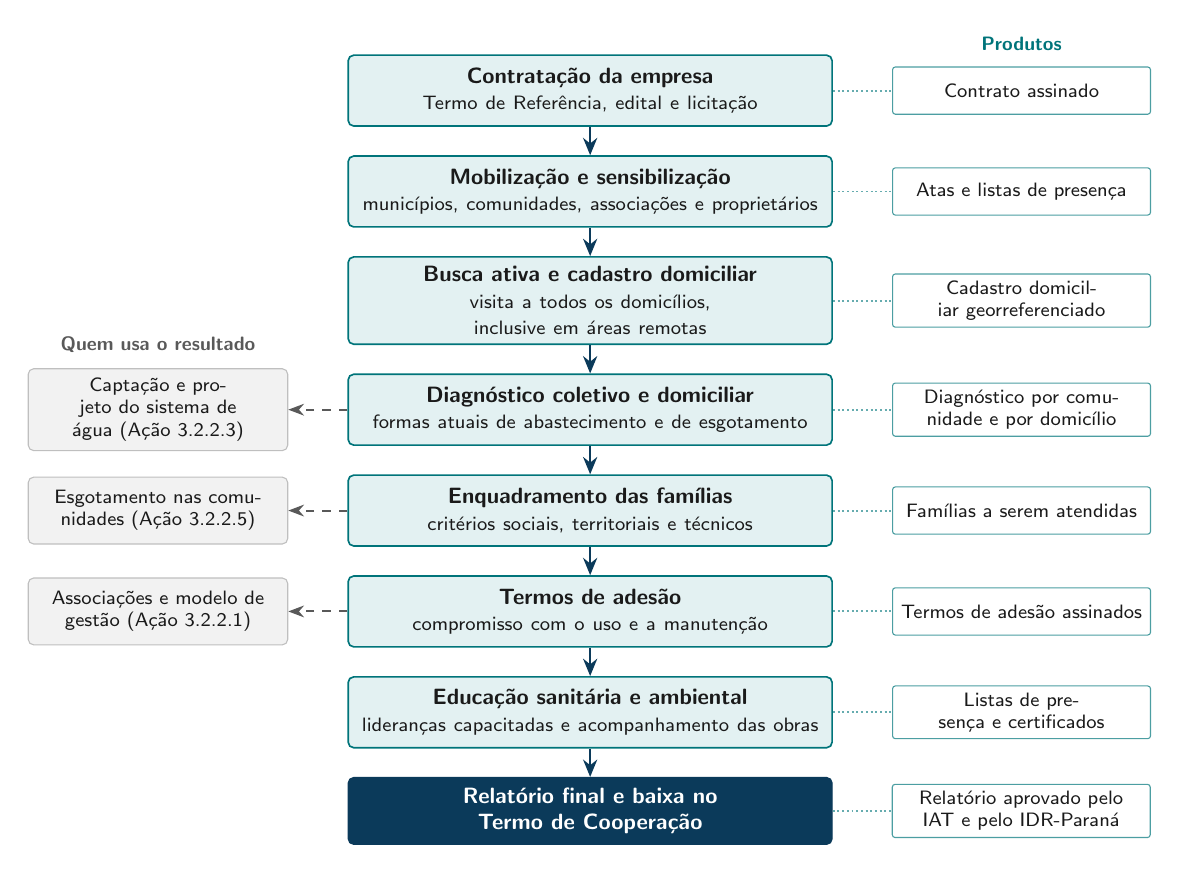
\begin{tikzpicture}[node distance=0.36cm,
    passo/.style={etapa=5.9cm, minimum height=0.9cm},
    liga/.style={draw=cTeal!60, densely dotted, line width=0.7pt}]
  \node[passo] (t1) {\textbf{Contratação da empresa}\\ {\scriptsize Termo de Referência, edital e licitação}};
  \node[passo, below=of t1] (t2) {\textbf{Mobilização e sensibilização}\\ {\scriptsize municípios, comunidades, associações e proprietários}};
  \node[passo, below=of t2] (t3) {\textbf{Busca ativa e cadastro domiciliar}\\ {\scriptsize visita a todos os domicílios, inclusive em áreas remotas}};
  \node[passo, below=of t3] (t4) {\textbf{Diagnóstico coletivo e domiciliar}\\ {\scriptsize formas atuais de abastecimento e de esgotamento}};
  \node[passo, below=of t4] (t5) {\textbf{Enquadramento das famílias}\\ {\scriptsize critérios sociais, territoriais e técnicos}};
  \node[passo, below=of t5] (t6) {\textbf{Termos de adesão}\\ {\scriptsize compromisso com o uso e a manutenção}};
  \node[passo, below=of t6] (t7) {\textbf{Educação sanitária e ambiental}\\ {\scriptsize lideranças capacitadas e acompanhamento das obras}};
  \node[marco=5.9cm, below=of t7] (t8) {Relatório final e baixa no Termo de Cooperação};
  \foreach \a/\b in {t1/t2,t2/t3,t3/t4,t4/t5,t5/t6,t6/t7,t7/t8}
    \draw[seta] (\a) -- (\b);

  \node[produto=3.1cm, right=0.75cm of t1] (q1) {Contrato assinado};
  \node[produto=3.1cm, right=0.75cm of t2] (q2) {Atas e listas de presença};
  \node[produto=3.1cm, right=0.75cm of t3] (q3) {Cadastro domiciliar georreferenciado};
  \node[produto=3.1cm, right=0.75cm of t4] (q4) {Diagnóstico por comunidade e por domicílio};
  \node[produto=3.1cm, right=0.75cm of t5] (q5) {Famílias a serem atendidas};
  \node[produto=3.1cm, right=0.75cm of t6] (q6) {Termos de adesão assinados};
  \node[produto=3.1cm, right=0.75cm of t7] (q7) {Listas de presença e certificados};
  \node[produto=3.1cm, right=0.75cm of t8] (q8) {Relatório aprovado pelo IAT e pelo IDR-Paraná};
  \foreach \a/\b in {t1/q1,t2/q2,t3/q3,t4/q4,t5/q5,t6/q6,t7/q7,t8/q8}
    \draw[liga] (\a) -- (\b);

  \node[externo=3.05cm, left=0.75cm of t4, font=\scriptsize] (u1) {Captação e projeto do sistema de água (Ação 3.2.2.3)};
  \node[externo=3.05cm, left=0.75cm of t5, font=\scriptsize] (u2) {Esgotamento nas comunidades (Ação 3.2.2.5)};
  \node[externo=3.05cm, left=0.75cm of t6, font=\scriptsize] (u3) {Associações e modelo de gestão (Ação 3.2.2.1)};
  \draw[setatracejada] (t4) -- (u1);
  \draw[setatracejada] (t5) -- (u2);
  \draw[setatracejada] (t6) -- (u3);
  \node[font=\scriptsize\bfseries, text=cTeal, above=0.08cm of q1] {Produtos};
  \node[font=\scriptsize\bfseries, text=cGrayText, above=0.08cm of u1] {Quem usa o resultado};
\end{tikzpicture}

\end{document}
